\documentclass[11pt, english]{article}

\usepackage{multicol}
\usepackage{hyperref}
\usepackage[eng]{felipito}
\usepackage{stfloats}
\usepackage{mathpazo}

\usepackage[margin=0.8in, left=0.7in, right=0.7in]{geometry}

\graphicspath{{./Graphics/}}

% Colors
\definecolor{urlcolor}{rgb}{0,.145,.698}
\definecolor{linkcolor}{rgb}{.71,0.21,0.01}
\definecolor{citecolor}{rgb}{.12,.54,.11}


% Document title
\title{\bf Problem Set 3 \\ Statistics, Computation and
Applications\\[-1ex]}
\author{Felipe del Canto}
\date{October, 2021}
    
\hypersetup{
	breaklinks=true,  % so long urls are correctly broken across lines
    colorlinks=true,
    urlcolor=urlcolor,
    linkcolor=linkcolor,
    citecolor=citecolor,
}

\begin{document}
    
\maketitle
   
\begin{multicols}{2}

\section*{Problem 3.1: The Manua Loa CO$_{2}$\\ concentration}

For part (a), the linear fit, its residuals and the ACF of the latter, are presented in \Cref{fig:co2-linear}. As can be seen from \Cref{fig:co2-linear-fit}, the linear model finds a upward trend ($\hat{\alpha}_{2} = 0.127$), consistent with the data. However, it does not seem adequate for modeling the trend in the data. The residuals plotted in \Cref{fig:co2-linear-res} confirm it. The image shows a strong U-shaped trend left in the residuals that is not accounted for in the linear model. In order to measure the goodness-of-fit of this model, in \Cref{fig:co2-linear-res-acf} is presented the autocorrelation function (ACF) of the residuals up to 40 lags. The image shows a positive and statistically significant correlation for the residuals with long-term dependencies. If the model was correctly specified, then we would expect at most a seasonality behavior that in the ACF would show as long-term dependencies and a ``symmetric'' plot with respect to 0.

\begin{figure*}[t]
	\caption{Linear trend fit, residuals and ACF of the residuals. The model was fitted using OLS.} \label{fig:co2-linear}
	\begin{subfigure}{0.45\textwidth}
		\caption{Linear fit} 
		\label{fig:co2-linear-fit}
		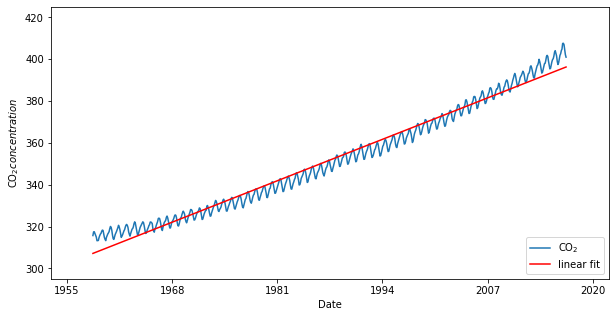
\includegraphics[width=\textwidth]{co2-linear-fit}
	\end{subfigure}\hfill
	\begin{subfigure}{0.45\textwidth}
		\caption{Residuals} 
		\label{fig:co2-linear-res}
		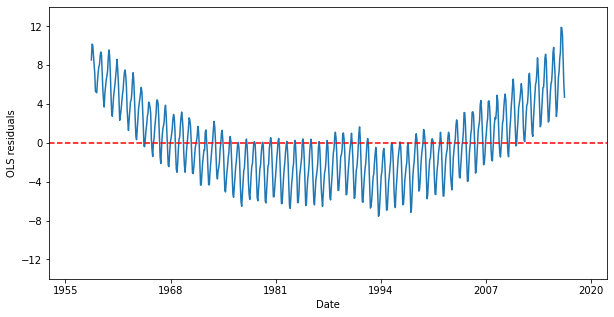
\includegraphics[width=\textwidth]{co2-linear-res}
	\end{subfigure}\vspace{2ex}
	\begin{subfigure}{0.5\textwidth}
		\centering
		\caption{ACF of residuals} 
		\label{fig:co2-linear-res-acf}
		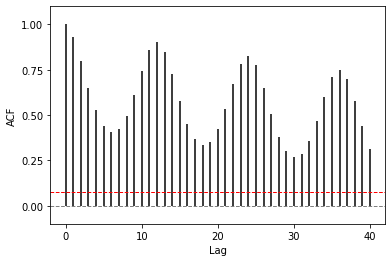
\includegraphics[width=0.8\textwidth]{co2-linear-res-acf}
	\end{subfigure}
\end{figure*}


\begin{figure*}[t]
	\caption{Quadratic trend fit and its residuals. The model was fitted using OLS.} \label{fig:co2-quadratic}
	\begin{subfigure}{0.45\textwidth}
		\caption{Quadratic fit} 
		\label{fig:co2-quadratic-fit}
		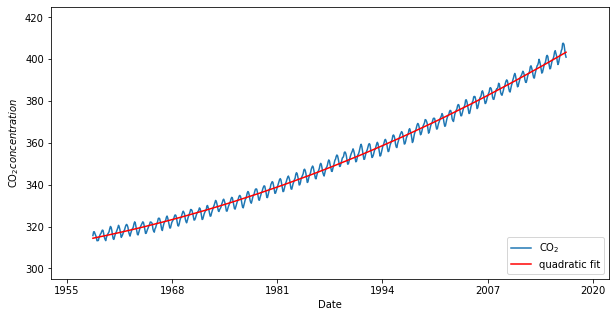
\includegraphics[width=\textwidth]{co2-quadratic-fit}
	\end{subfigure}\hfill
	\begin{subfigure}{0.45\textwidth}
		\caption{Residuals} 
		\label{fig:co2-quadratic-res}
		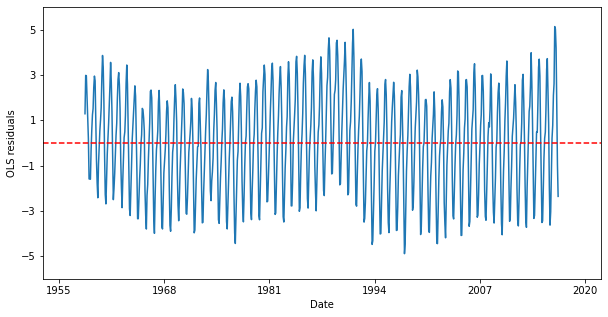
\includegraphics[width=\textwidth]{co2-quadratic-res}
	\end{subfigure}\vspace{2ex}
	\begin{subfigure}{0.5\textwidth}
		\centering
		\caption{ACF of residuals} 
		\label{fig:co2-quadratic-res-acf}
		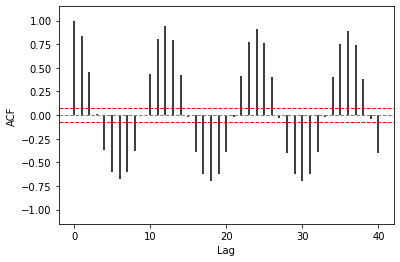
\includegraphics[width=0.8\textwidth]{co2-quadratic-res-acf}
	\end{subfigure}
\end{figure*}

\begin{figure*}[t]
	\caption{Quartic trend fit and its residuals. The model was fitted using OLS.} \label{fig:co2-quartic}
	\begin{subfigure}{0.45\textwidth}
		\caption{Quartic fit} 
		\label{fig:co2-quartic-fit}
		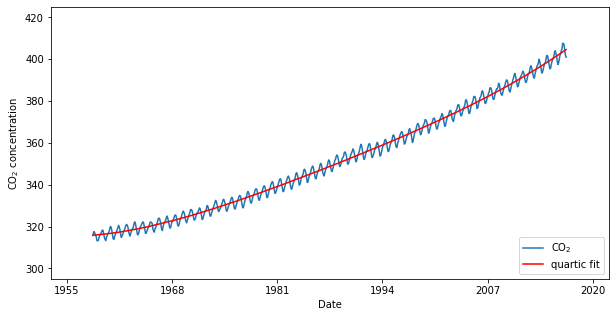
\includegraphics[width=\textwidth]{co2-quartic-fit}
	\end{subfigure}\hfill
	\begin{subfigure}{0.45\textwidth}
		\caption{Residuals} 
		\label{fig:co2-quartic-res}
		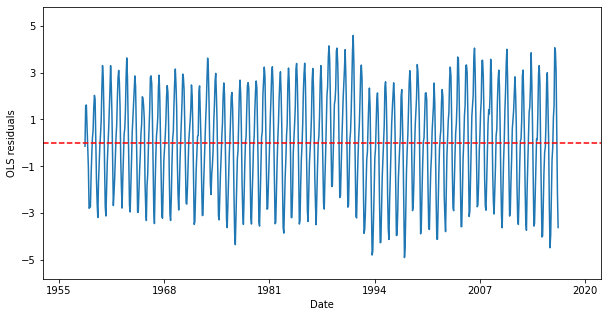
\includegraphics[width=\textwidth]{co2-quartic-res}
	\end{subfigure}\vspace{2ex}
	\begin{subfigure}{0.5\textwidth}
		\centering
		\caption{ACF of residuals} 
		\label{fig:co2-quartic-res-acf}
		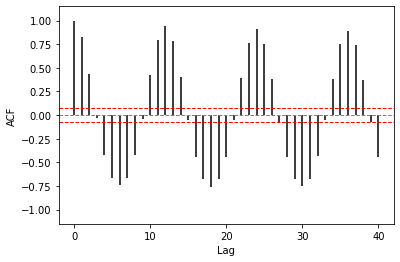
\includegraphics[width=0.8\textwidth]{co2-quartic-res-acf}
	\end{subfigure}
\end{figure*}


For part (b), I repeat the same experiment as in part (a), but with a quadratic model. The corresponding results are presented in \Cref{fig:co2-quadratic}. In this case, the fit diminishes the coefficient of $t$ ($\hat{\beta}_{2} = 0.065$), but includes a small convexity ($\hat{\beta}_{3} = 8.692 \cdot 10^{-5}$). The residual plot in \Cref{fig:co2-quadratic-res} shows that the previous U-shaped trend present in the linear fit has dissapeared. However, there still persists an anomaly around 1990 that might correspond to a residual trend not captured by the model. In terms of the goodness-of-fit, the ACF in \Cref{fig:co2-quadratic-res-acf} shows that now the dependencies between residuals are much shorter and the graph is mostly symmetric around 0. This suggests this model is a much better fit than the linear one.

For part (c), I repeat the previous experiments using a quartic model. The corresponding results are presented in \Cref{fig:co2-quartic}. The differences of this model with respect to the quadratic one are small. However, some features are salient. For example, in \Cref{fig:co2-quartic-res} it can be seen that the small variations across time are almost eliminated. What is more, the ACF in \Cref{fig:co2-quartic-res-acf} exhibits a slightly more symmetric shape, with negative correlations closer to -1, showing that the trend is better captured with this model. Nevertheless, this improvements are really small and the coefficients associated with $t^{3}$ and $t^{4}$ have orders of magnitude too small ($10^{-7}$ and $10^{-10}$, respectively) to consider this model a much better fit than the quadratic one. In general terms, a higher order model will always be able to improve the fit with respect to a lower order one. This, since models with order $n$ are particular cases of models of order $m > n$, where the coefficients for $t^{k}$ with $k > n$ have been set to 0. However, since the objective is to capture a trend in the data and not fit the data itself, then I would consider increasing the order of the model until there is no apparent trend in the residuals. The latter can be detected visually by plotting the residuals, or through an ACF.

For part (d), the monthly average of the residuals in \Cref{fig:co2-quadratic-res} is presented in \Cref{fig:co2-montly-res-average}. The picture shows a strong seasonal component that varies month by month. In \Cref{fig:co2-season-adj} is presented the time series with this seasonality extracted, compared with the provided season-adjusted series. From the image, there is no apparent difference between both corrections. 

\begin{figure*}[t]
	\centering
	\caption{Monthly average of residuals of quadratic model.}
	\label{fig:co2-montly-res-average}
	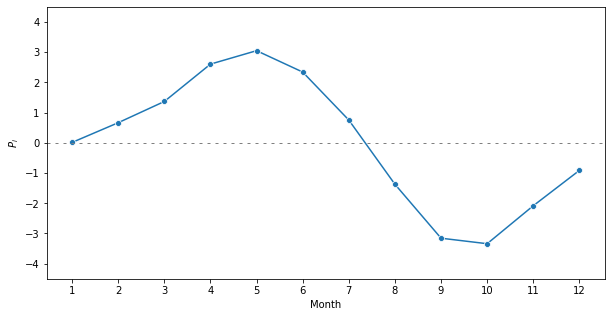
\includegraphics[width=0.5\textwidth]{co2-montly-res-average}
\end{figure*}

\begin{figure*}[b]
	\centering
	\caption{Deseasoned Manua Loa series. In red, the adjustment was made using the monthly average of the quartic fit residuals. In blue, the provided adjustment.}
	\label{fig:co2-season-adj}
	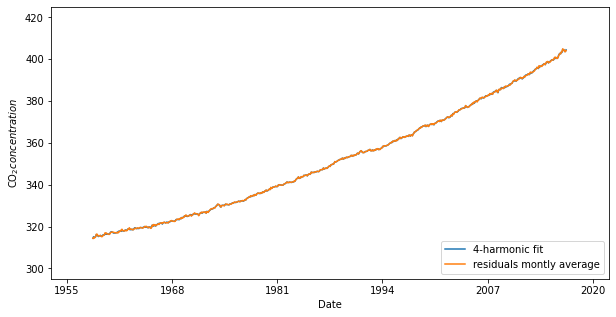
\includegraphics[width=0.5\textwidth]{co2-season-adj}
\end{figure*}

For part (e), in \Cref{fig:co2-seasonal-quadratic-fit} is presented the quadratic fit with the seasonality in \Cref{fig:co2-montly-res-average} incorporated. In general terms, the CO$_{2}$ concentration shows an upward trend with a monthly seasonal behavior. The upward trend in consistent with the increase in pollutants that we are observing around the globe and the environmental consequences therein. In particular, the global warming phenomenon is consistent with an increase in the concentrations of CO$_{2}$ in the atmosphere. On the other hand, the seasonality observed may be correlated with the temperature, which changes depending on the season of the year. Under this argument, lower temperatures correlate with higher concentrations of CO$_{2}$, since it is more difficult for this gas to escape the atmosphere when temperatures are low (low kinetic energy). On the other hand, when temperatures start to rise, more CO$_{2}$ is capable of escaping the atmosphere and consequently, the concentration is lower. Finally, in \Cref{fig:co2-seasonal-fit-residuals} are presented the residuals of this quadratic fit with seasonal component. The resulting series looks more or less stationary. However, the ACF of the residuals of this series (see \Cref{fig:co2-residual-series-acf}) is not consistent with a stationary series, where long-term correlations should fade.

\begin{figure*}
	\centering
	\caption{Quadratic fit with seasonal component, its residuals, and the ACF of the residuals.}
	\label{co2-seasonal-fit}
	\begin{subfigure}{0.45\textwidth}
		\caption{Quadratic fit with seasonal component}
		\label{fig:co2-seasonal-quadratic-fit}
		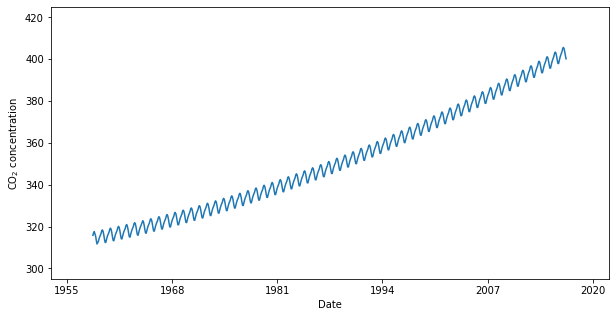
\includegraphics[width=\textwidth]{co2-seasonal-quadratic-fit}
	\end{subfigure}\hfill
	\begin{subfigure}{0.45\textwidth}
		\caption{Residuals}
		\label{fig:co2-seasonal-fit-residuals}
		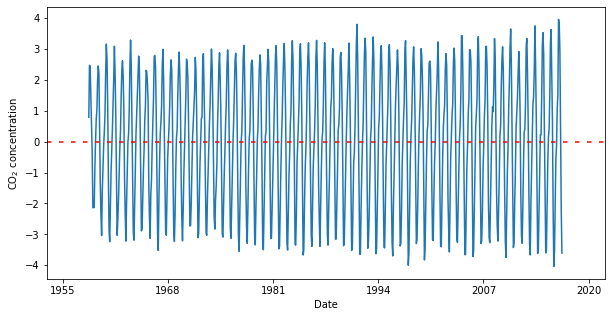
\includegraphics[width=\textwidth]{co2-seasonal-fit-residuals}
	\end{subfigure}\vspace{2ex}
	\begin{subfigure}{0.45\textwidth}
		\centering
		\caption{ACF of residuals}
		\label{fig:co2-residual-series-acf}
		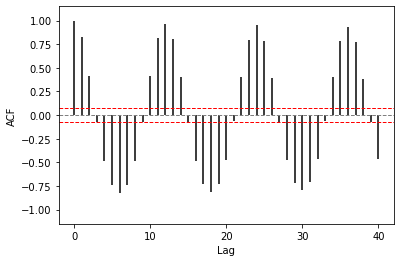
\includegraphics[width=0.85\textwidth]{co2-residual-series-acf}
	\end{subfigure}
\end{figure*}


\section*{Problem 3.2: PPP Data Analysis}
  
For this problem, the first step is to construct the database. After loading the data, the first step is to keep the relevant observations. In this case, for both the \texttt{CPI} and \texttt{PriceStats} variables, the relevant values will be those of the first of each month. Additionally, the monthly averages of both variables will be stored. After this, the $\log$ of all 4 variables is computed. This, in order for these variables to have the same units as the BER rates.

After this, the next step is to merge this dataset with the ones that include the BER for 5 and 10 years. In this case also the first month value and monthly averages are stored. Consequently, after these steps, the final dataset contains 8 variables.
 
For part (a), since the idea is to predict the values of the CPI (in order to predict inflation), the first step is to choose an appropriate model. For this data generating process, the best option is an AR model. The reason behind this is that prices have a persistent property, in the sense that prices at time $t$ are good reflections for prices in $t+1$, since consumers base their decisions in those prices. Instead, an MA model, for example, will have some persistency but this is not structural to the model. Consider an MA(1) model. In this case, $X_{t} = W_{t} + \theta W_{t-1}$ and, consequently, $X_{t+1}$ will also depend on $W_{t}$. However, the main rationale is that prices are correlated \textit{with each other} and not only trough with their underlying generation process.

Now, in order to determine the best AR model, the PACF plot is useful. In \Cref{fig:PACF-cpi}, it is possible to observe a sharp decline in the PACF after lag 1. In fact, from lags 2 to 20, the estimates fall within the 95\% confidence interval around 0. Consequently, the image suggests that an AR(1) model may be a good fit for this data. The point estimate for the lagged term in this model is very close to 1 ($\hat{\phi}_{1} = 0.9983$) and for this reason the predictions of this model look very similar to the original series, lagged by one month (see \Cref{fig:cpi-ar-fit}). The MSPE for this model is $1.571 \cdot 10^{-5}$. It is interesting to note that, even if the AR(1) model is suggested by the PACF, this is not the one that incurs in the lowest prediction error. In that regard, testing the predictions of AR($k$) models with $1 \leq k \leq 10$ resulted in a minimum MSPE of $1.038\cdot 10^{-5}$, when $k = 3$. Most notably, the MSPE is not monotone in the order of the model.

\begin{table*}[b]
	\centering
	\caption{MSPE for AR(1) prediction models. The dependent variable is the $\log$ CPI and the exogenous regressors are the $\log$ of PriceStats, and the 5 and 10 years BER. These last variables are considered with their first-day value and the monthly average. All values are rounded to the nearest hundredth.}
	\label{tab:part-c-estimates}
	\begin{tabular}{cccccc}
		\hline\hline
		\\[-1.8ex]
		&Exogenous regressors	&	Type 			&	Linear trend	&	Seasonal Trend	&	MSPE	\\[0.5ex]\hline
		\\[-1ex]
		\multicolumn{6}{l}{\small\textit{Panel A: AR(1) (base specification)}}											\\
		&	\xmark				&	\xmark			&	\xmark			&	\xmark			&	$1.57 \cdot 10^{-5}$	\\[0.5ex]
		\\[-1ex]
		\multicolumn{6}{l}{\small\textit{Panel B: AR(1) with exogenous regressors}}	\\
		&	\cmark				&	First-day		&	\xmark			&	\xmark			&	$6.20 \cdot 10^{-6}$	\\[0.5ex]
		&	\cmark				&	Monthly average	&	\xmark			&	\xmark			&	$6.63 \cdot 10^{-6}$	\\[0.5ex]
		\\[-1ex]
		\multicolumn{6}{l}{\small\textit{Panel C: AR(1) with exogenous regressors and trends}}	\\
		&	\cmark				&	First-day		&	\cmark			&	\xmark			&	$7.48 \cdot 10^{-6}$	\\[0.5ex]
		&	\cmark				&	First-day		&	\xmark			&	\cmark			&	$6.40 \cdot 10^{-6}$	\\[0.5ex]
		&	\cmark				&	First-day		&	\cmark			&	\cmark			&	$8.01 \cdot 10^{-6}$	\\[0.5ex]
		\hline\hline
	\end{tabular}
\end{table*}

\begin{figure*}[b]
	\centering
	\caption{Partial auto-correlation function plot for the $\log$ of the Consumer Price Index. The red lines correspond to the 95\% confidence interval around 0.}
	\label{fig:PACF-cpi}
	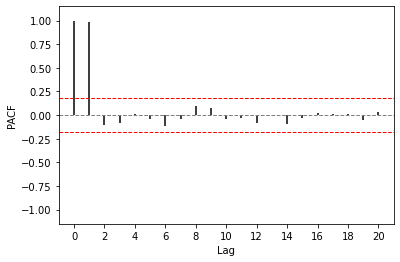
\includegraphics[width=0.5\textwidth]{PACF-cpi}
\end{figure*}

\begin{figure*}[b]
	\centering
	\caption{$\log$ CPI (in blue) and AR(1) model fit (in red). Since the point estimate for the model is 0.9983, the predicted series looks similar to the original, lagged by one term.}
	\label{fig:cpi-ar-fit}
	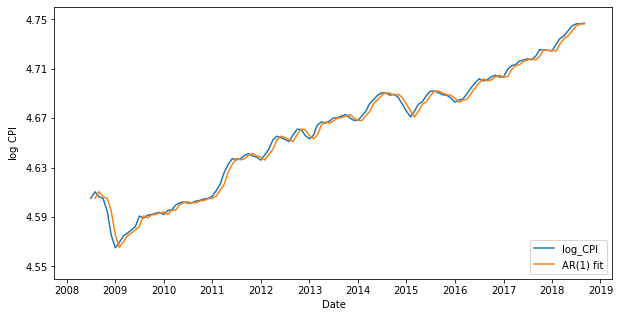
\includegraphics[width=0.6\textwidth]{cpi-ar-fit}
\end{figure*}

\begin{figure*}[b]
	\centering
	\caption{Inflation rate predictions using the AR(1) fit, the PriceStats data, and the 10 and 5 year maturity BER. For this last variable, the first-day value and monthly averages are used.}
	\label{fig:inflation-estimates}
	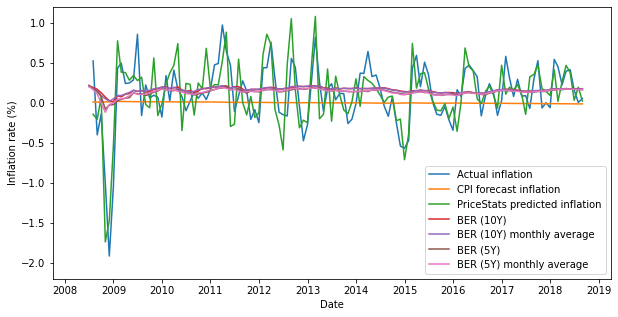
\includegraphics[width=0.6\textwidth]{inflation-estimates}
\end{figure*}

\begin{figure*}[b]
	\centering
	\caption{$\log$ CPI (in blue) and AR(1) model fits. The AR(1) model includes the exogenous regressors $\log$ PriceStats, and the 5 and 10 year BER. For these last two variables, the first-day value (in red) and monthly averages (in green) are considered.}
	\label{fig:cpi-part-d-fit}
	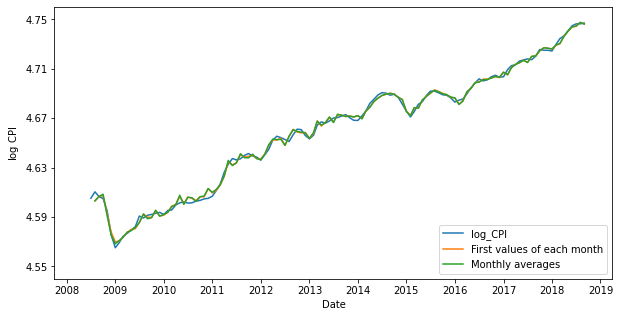
\includegraphics[width=0.6\textwidth]{cpi-part-d-fit}
\end{figure*}


For part (b), in order to estimate the inflation rate, all the variables in the dataset are used. Based on the AR(1) predictions, the inflation rate in month $t$, $\pi_{t}$ is computed as follows:
	\begin{equation} \label{eq:inflation-cpi}
		\pi_{t} = \left(\frac{\widehat{CPI}_{t}}{CPI_{t-1}} - 1\right) \cdot 100,
	\end{equation}
where $\widehat{CPI}_{t}$ is the estimated CPI in month $t$, using the previous AR(1) model. Using the PriceStats data, the inflation rate is computed as:
	$$\pi_{t} = \left(\frac{\text{PriceStats}_{t}}{\text{PriceStats}_{t-1}} - 1 \right) \cdot 100$$
Finally, since the BER rate is a proxy for the annual inflation rate, the monthly inflation rate is obtained by dividing the BER by 12. This is done for both the first-day value and the monthly average. The inflation estimates are shown in \Cref{fig:inflation-estimates}. As expected, the CPI forecasts predicted inflation is close to zero. This, because the AR(1) model sets the prediction for the next month almost equal to the previous one (and thus the fraction in (\ref{eq:inflation-cpi}) is almost 1. Interestingly, the PriceStats predicted inflation is actually very close to the actual inflation. This is expected, since the variable is not being forecasted.

On the other hand, the BER prediction power its low, mostly because this rate is concerned with future (average) inflation rates and thus is much smoother than the actual inflation rate. However, it codes expectations (which are crucial to price determination) and thus will be helpful in obtaining better estimates for part (c).

For part (c), to improve the inflation predictions, the AR(1) model in (b) will include exogenous regressors. The idea is that, if the model accurately predicts the next month CPI, then it accurately predicts the inflation rate (see \ref{eq:inflation-cpi})In particular, the data from PriceStats and the BER will be included. This will be done in two ways: using the first-day values and the monthly averages. The predicted series and MSPE are presented in \Cref{fig:cpi-part-d-fit} and \Cref{tab:part-c-estimates}, panel B, respectively. The inclusion of these regressors reduces the prediction error in one order of magnitude. It is worth noting that using the monthly averages (instead of the first values of each month) also improves the first prediction (with a MSPE of $6.63 \cdot 10^{-6}$) but it is not as good as using the first values of each month. The reason behind this behavior might be that monthly averages tend to smooth a phenomenon that is highly noisy. Consequently, inflation rates obtained by averaging tend to have a higher prediction error.

For part (d), the same AR(1) model with first-day values used in (c), but including (i) seasonal corrections, (ii) a linear trend, and (iii) both, where fitted. The results are shown in \Cref{tab:part-c-estimates}, panel C. It is interesting to note that none of the three models considered are capable of improving the first-day AR(1) model of panel B. This may be due to deterministic trends having to much incidence in the prediction, meaning less flexibility.

For part (e), to compute the ACF, note that if $h \geq 2$, then $X_{t}$ and $X_{t+h}$ have no $W_{\tau}$ terms in common. Since $\{W_{t}\}$ are independent, then this implies
	$$\gamma(h) := \mathrm{Cov}(X_{t+h}, X_{t}) = 0,\qquad h \geq 2.$$
Thus, the only relevant covariances to compute are the ones with $h=1$ and $h=0$. For $h=1$, we have
	$$\gamma(1) = \mathrm{Cov}(W_{t+1} + \theta W_{t}, W_{t} + \theta W_{t-1}).$$
Using the fact that the $W_{t}$ are independent, then
	$$\gamma(1) = \theta \mathrm{Cov}(W_{t}, W_{t}) = \theta\sigma^{2}.$$
Finally, for $h =0$,
	\begin{align*}
		\gamma(0)	&=	\mathrm{Cov}(W_{t} + \theta W_{t-1}, W_{t} + \theta W_{t-1})	\\
					&=	(1+\theta^{2})\sigma^{2}
	\end{align*}
In terms of the mean for this model, we have
	$$\mathbb{E}(X_{t}) = \mathbb{E}(W_{t} + \theta W_{t-1}).$$
And since $W_{t}, W_{t+1}$ are independent and have zero mean, then
	$$\mathbb{E}(X_{t}) = 0$$

Altogether, this implies that a time series under a MA(1) model is a zero-mean series whose ACF at lag 0 is equal to $(1+\theta^{2})\sigma^{2}$ and at lag 1 is equal to $\theta \sigma^{2}$. At lags $h \geq 2$, the ACF should be zero. In particular, if $\theta < 0$, then the ACF is positive at lag 0 and negative at lag 1.

For part (f), let $h > 0$ and $\gamma(h) = \mathrm{Cov}(X_{t+h}, X_{t})$, which is independent of $t$ since $X_{t}$ is stationary. We have that
	\begin{align*}
		\gamma(h)
			&=	\mathrm{Cov}(X_{t+h}, X_{t})	\\
			&=	\mathrm{Cov}(\phi X_{t+h-1} + W_{t+h}, X_{t})	\\
			&=	\phi \gamma(h-1) + \mathrm{Cov}(W_{t+h}, X_{t})
	\end{align*}
Since $X_{t}$ is independent from $W_{t+h}$ for $h > 0$, then
	$$\gamma(h) = \phi \gamma(h-1)$$
And thus
	$$\gamma(h) = \phi^{h}\gamma(0)$$
In order to obtain $\gamma(0)$, note that,
	\begin{align*}
		\gamma(0)	&=	\mathrm{Cov}(X_{t}, X_{t})	\\
					&=	\mathrm{Cov}(\phi X_{t-1} + W_{t}, \phi X_{t-1} + W_{t})	\\
					&=	\phi^{2} \gamma(0) + \sigma^{2}
	\end{align*}	
And thus
	$$\gamma(0) = \frac{\sigma^{2}}{1-\phi^{2}}$$
Which implies that
	$$\gamma(h) = \frac{\phi^{h}}{1-\phi^{2}}\, \sigma^{2}$$

Finally, let $\mu := \mathbb{E}(X_{t})$. Using stationarity, we have that
	\begin{align*}
		\mu	&=	\mathbb{E}(X_{t})	\\
			&=	\mathbb{E}(\phi X_{t-1} + W_{t})	\\
			&=	\phi \mu
	\end{align*}
And thus,
	$$(1-\phi)\mu = 0$$
Since $|\phi| < 1$, then $\mu = 0$. In particular, the AR(1) model has the same mean as any MA($q$) model. However, note that for the AR(1) model, $\gamma(h)\neq 0$ for all $h$, whereas an MA($q$) model has $\gamma(h) = 0$ for $h > q$. To fix this, consider the following MA($\infty$) model
	$$X_{t} = \sum_{s=0}^{\infty} \theta^{s}W_{t-s},$$
where $|\theta| < 1$, and $W_{t} \overset{iid}{\sim} WN(0,\sigma^{2})$. Observe that,
	\begin{align*}
		X_{t}
			&=	W_{t} + \theta\sum_{s=0}^{\infty} \theta^{s} W_{(t-1)-s}	\\
			&=	\theta X_{t-1} + W_{t}
	\end{align*}
which means that this model is an AR(1) model. This proves that an AR(1) model is the limit when $q \to \infty$ of a MA($q$) model.


\end{multicols}
\end{document}
